\chapter{Developer documentation}
\label{ch:impl}

In this chapter, we are going to get into details about the software architecture,
the solutions to certain problems encountered during implementation and how everything came up together in the end.
\\[5pt]
In order to build and run the application as a developer, you must follow the same steps as in \ref{s:installation_guide}.
\\[5pt]
As it was mentioned before the application is completely connected to \textbf{Mastodon} \cite{test}. So, it is useless and
not the correct way to use it without using Mastodon.




\section{Mastodon API}\label{s:api}
As it was mentioned in \ref{s:project_desc}, this application checks whether an account
that is trying to reach you is a possible threat or not. To do this check we need the data
of the account. So, we have to connect to an API that gets the data from
the live Mastodon server in order to check the possibility of a threat account.
In addition, the API is used to let us take the actions mentioned in \ref{s:Actions_threat}
directly from our application, without the need of doing it through Mastodon.
For this application we used an already created API for Python called
\textbf{Mastodon API}  \cite{apimast}.
\\[5pt]
Below we can see a scheme of how this API operates.
\\[5pt]
\begin{figure}[H]
	\centering
	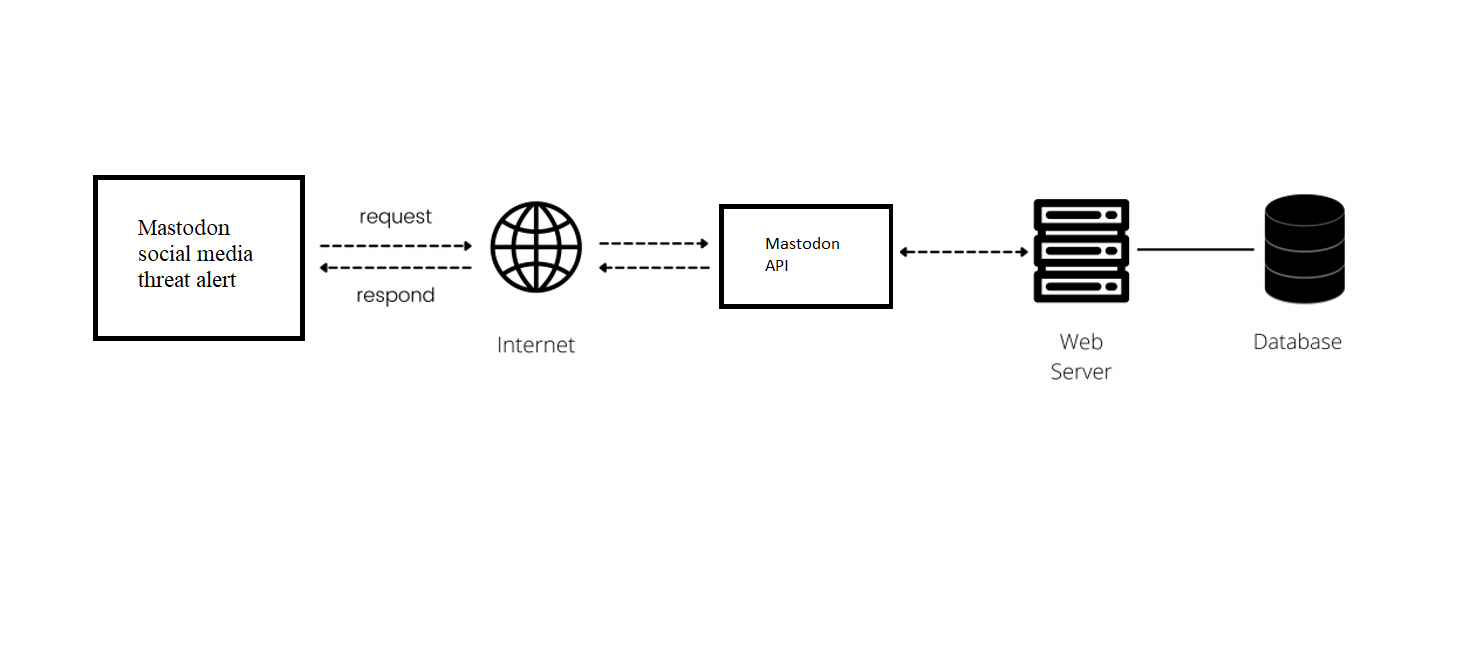
\includegraphics[width=1.0\textwidth,height=200px]{images/MastodonApi.png}
	\caption{Mastodon API scheme}
	\label{fig:mast_api}
\end{figure}
\subsection{API rate limits}\label{ss:rate_lim}
This API has a fixed rate-limit that is 300 requests per 5 minutes, in order not to
violate the rate-limit and not make the user wait for 5 minutes until the rate-limit resets, we
needed to get data from the live server every 2.6 second so the user can get the full
experience of Mastodon. This being said, the user has enough time to surf the feed without having
to wait for 5 minutes.
\subsection{API initialization}\label{ss:api_init}
To use this API we need to use the user's credentials to log into Mastodon account through the API, and those credentials will be saved in \textit{.secret} files in the directory where we call the API, and that is the reason why the user must give the credentials in the starting window of the application. Below are the methods required to call in order to log into the Mastodon account through the API.
\\[5pt]
\begin{lstlisting}[language=python, caption={Logging in to Mastodon account through the API}, captionpos=b ]
	def __init__(self):
		self._user = Mastodon()
		self._userApiInstance = Mastodon()
		self._mastodonServer = ""
	
	def createApp(self, mastodon_server):
		if(mastodon_server.split("://")[0] != "https"):
			self._mastodonServer = "https://" + mastodon_server
		else:
			self._mastodonServer = mastodon_server
	
	Mastodon.create_app(
		"mastodonApiAppUser",
		api_base_url=self._mastodonServer,
		to_file='app/secretFolder/mastodonApiAppUser.secret'
	)
	
	def setUpAccounts(self):
		self._user = Mastodon(
			client_id='app/secretFolder/mastodonApiAppUser.secret',
			api_base_url=self._mastodonServer
		)
	
	def loginAccount(self, username, password, user=True):
		if user:
			self._user.log_in(
				username,
				password,
				to_file='app/secretFolder/usercredentials.secret' 
			)
\end{lstlisting}
\subsection{API instance}\label{ss:api_instance}
Logging in to the account is not enough in order to use this API, but we can say it is a very important step and a must. To actually start using the API we need to create an API instance for that account. Below you can see the method that creates the API instance for both, user account or admin account.
\\[5pt]
\begin{lstlisting}[language=python, caption={Creating API instance}, captionpos=b]
	def createApiInstance(self):
		self._userApiInstance = Mastodon(
				access_token='app/secretFolder/usercredentials.secret',
				api_base_url=self._mastodonServer
		)
\end{lstlisting}
So, we have to create an access token from the user credentials saved in \textit{.secret} file, and after creating the API instance we can start using the API methods. The main methods that this application uses are:
\begin{itemize}
	\item \textbf{Get the notifications}
	\item \textbf{Clear the notifications}
	\item \textbf{Block an account}
	\item \textbf{Block a domain}
	\item \textbf{Get a certain account's data}
	\item \textbf{Get user's following accounts}
	\item \textbf{Mute an account}
\end{itemize}
We will deep dive into each of the methods in the following sections.
\subsection{Notifications}\label{ss:notif}
To get the accounts that are trying to reach the user, we first need to get the notifications and filter them to only get the direct messages and tags, which is done
by setting the parameter named \textbf{mentions\_only} to true.
To get the notifications through the API we can use the following method:
\\[5pt]
\begin{lstlisting}[language=python, caption={Getting the notifications by API}, captionpos=b]
	def getNotifications(self):
		return self._userApiInstance.notifications(mentions_only=True)
\end{lstlisting}
And in order to filter them we need to go through each and filter them by their type and existence in the application's database.
\\[5pt]
\begin{lstlisting}[language=python, caption={Filtering the notifications}, captionpos=b]
	def startSession(self):
		try:
			notifications = self.api.getNotifications()
			accounts_reaching_user = []
			for notification in notifications:
				account_id = notification['account']['id']
				
				inDatabase = self.isAccountInDatabase(int(account_id))
		
				if (account_id not in accounts_reaching_user and not inDatabase):
					accounts_reaching_user.append(account_id)
	
			return accounts_reaching_user
		except Exception:
			return []
\end{lstlisting}
\subsection{Getting account's data}\label{ss:acc_data}
As it was mentioned in \ref{s:api} we need to get the account's data in order to check for the possibility of the threat. To get the data of a certain account, we need that account's id and we can get the public data for that account such as:
\begin{itemize}
	\item \textbf{Account ID}
	\item \textbf{Username}
	\item \textbf{Domain}
	\item \textbf{Followers Count}
	\item \textbf{Followings Count}
	\item \textbf{Statuses count}
	\item \textbf{Avatar}
	\item \textbf{Header}
	\item \textbf{Date of creation}
\end{itemize}
And in order to fetch those data we can simply call the API method which is as below:
\\[5pt]
\begin{lstlisting}[language=python, caption={Fetching certain account's public data}, captionpos=b]
	def getAccountData(self, account_id, admin=False):
		if not admin:
			return self._userApiInstance.account(account_id)
\end{lstlisting}
This method will return the data as a dictionary where the keys are the public data names and the values are their values.
\subsection{Getting user's following accounts}
We know that if we follow someone that means we most probably know him/her. Hence, we need to trust the accounts we follow when we start our application. To trust them we need to get the list of the accounts we follow, which is done by the following method:
\\[5pt]
\begin{lstlisting}[language=python, caption={Method to get the list of the accounts we follow}, captionpos=b]
	def getFollowingAccounts(self):
		my_id = self._userApiInstance.me()['id']
		return self._userApiInstance.account_following(my_id)
\end{lstlisting}
As we can see, we first need to get our account id and then get the list of the accounts we follow. After having the list of the accounts we follow, we need to trust by inserting each in the application's database so we don't have to check them if they try to reach us.
\\[5pt]
\begin{lstlisting}[language=python, caption={Inserting the accounts we follow immediately in the application's database}, captionpos=b]
	def trustFollowings(self):
		following_accounts = self.api.getFollowingAccounts()   
		for account_data in following_accounts:
			try:
				account_id = int(account_data['id'])
				username = str(account_data['username'])
				domain = str(account_data['url'].split('/')[2])
				self.__database.insertAccount(account_id, username, domain, False)
				self.__database.insertDomain(domain, False)
			except Exception:
				print("Error")
\end{lstlisting}
\subsection{Blocking an account}
As it was mentioned in \ref{ss:act_action} we have the option to block an account and of course the only way to do it outside the application is by using the API. So, in order to block an account we need to call the API method and pass the account's id as a parameter
and the account with that id will be blocked.
\\[5pt]
\begin{lstlisting}[language=python, caption={Blocking an account method}, captionpos=b]
	def blockAccount(self, account_id):
		self._userApiInstance.account_block(account_id)
		return True
\end{lstlisting}
\subsection{Muting an account}
Same as blocking an account, when we want to mute a certain account we need to call the API method and pass the account's id as a parameter.
\\[5pt]
\begin{lstlisting}[language=python, caption={Muting an account method}, captionpos=b]
	def muteAccount(self, account_id):
		self._userApiInstance.account_mute(account_id)
		return True
\end{lstlisting}
\subsection{Blocking a domain}
When it comes to blocking a domain the parameter changes, since the domains are not classified with ids. If we want to block a domain we need to pass the domain's name as a parameter, but keep in mind that the domain is case-sensitive.
\\[5pt]
\begin{lstlisting}[language=python, caption={Blockin a domain method}, captionpos=b]
	def blockDomain(self, domain):
		self._userApiInstance.domain_block(domain)
		return True
\end{lstlisting}

\section{Predictive Model}\label{s:model}
Classifying the possibility of a threat is done by a machine learning predictive model.
To create our model we used the \textbf{Scikit-learn} \cite{scikit-learn} Python library, to
preprocess the data we used \textbf{Pandas} \cite{pandas} Python library and in order to save the
model so it doesn't need to go through the training process again we used \textbf{Pickle} \cite{pickle}
\\[5pt]
Since our problem was to classify whether an account has a possibility of being a threat,
we had to choose between the classification algorithms. Considering multiple factors and trying
multiple algorithms we chose to go with Logistic regression for these main reasons:
\begin{itemize}
	\item \textbf{Small dataset}, Logistic regression is known to give the best results in small datasets.
	\item \textbf{Low complexity model}, since we had to classify between two classes and we had 19 features to consider,
	we needed to use a low complexity model.
\end{itemize}
\subsection{Data preprocessing}
As it was mentioned above we had to deal with data preprocessing in order to make our dataset suitable
to train the model. We needed to read the data from a csv file and create a dataset based on the data
that was available on that file. The file contained accounts with account's data and it has already classified all of them as threat
and not threat. However, we didn't get all the account's data since some of them were not related to our problem, such as username, account id etc.
It is worth mentioning that we considered the following account's data only:
\begin{itemize}
	\item \textbf{Followers count}, the number of the accounts that follow the account.
	\item \textbf{Followings count}, the number of the accounts that the account follows.
	\item \textbf{Statuses count}, the number of the statuses the account has posted.
	\item \textbf{Profile picture}, whether the account has a profile picture.
	\item \textbf{Domain}, account's Mastodon domain.
	\item \textbf{Year of creation}, the year when the account was created.
\end{itemize}
As we can see we had some of the data in string format, like year of creation and domain, so we
had to use the dummy encoder from Pandas and that limited our range of domains and year of creation.
So, now the model recognized only the following domains:
\begin{itemize}
	\item \textbf{mastodon.elte.hu}
	\item \textbf{mastodon.social}
	\item \textbf{mastodon.technology}
	\item \textbf{mastodon.xyz}
	\item \textbf{scholar.social}
	\item \textbf{fosstodon.org}
	\item \textbf{hofelho.hu}
\end{itemize}
About the year range, we thought that it was more than enough to consider accounts created from 2015, since
the older the account, the less the possibility of being a threat is.
So, after applying the dummy encoder our features increased from 6 to 19.
\\[5pt]
Since some of our data could get big values, like the followers count and following count, we needed
to apply normalization on data, so that we could get more accurate predictions in the end.
After normalization we split the dataset into training set and testing set, where 70 percent of the data was on the
training set and the other 30 percent of the data was on the testing set.
\subsection{Exploratory data analysis - EDA}
During our EDA we found out that we have some outliars in our dataset, but the number was quite low, somewhere from 4 to 7
in total. Hence, we didn't remove the outliars since the number was very low and it didn't affect the training dataset.
\\[5pt]
Besides outliars, we didn't have any null value in the fields we used to train, which made our EDA process less complex
since we didn't have to deal with null values.
\\[5pt]
One important thing that is worth mentioning is that we discovered a pattern that showed us that if an account has
way more followings than followers, doesn't have a profile picture or the followings count is very low, ranging from 0 to 4, the
chances for that account to be a possible threat were higher.
\subsection{Model performance}
We mentioned in \ref{s:model} that we needed a low complexity algorithm, and we know that we have three different kinds
provided by Scikit-learn which are:
\begin{itemize}
	\item \textbf{Logistic regression}
	\item \textbf{SVC}
	\item \textbf{Naive Bayes}
\end{itemize}
After trying each of the algorithms, we wanted to go with Logistic regression since the performance, confusion matrix
and the ROC curve was showing us that Logistic regression is performing better in comparison to the other two.
\\[5pt]
\begin{figure}[H]
	\centering
	\subcaptionbox{Naive Bayes performance scores}{
		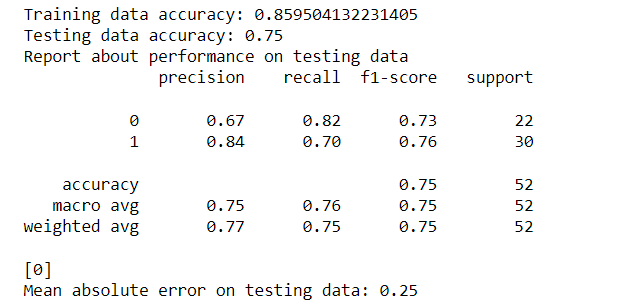
\includegraphics[width=0.45\textwidth, height=130px]{images/naivebayesperf.png}}
	\hspace{5pt}
	\subcaptionbox{Naive Bayes confusion matrix}{
		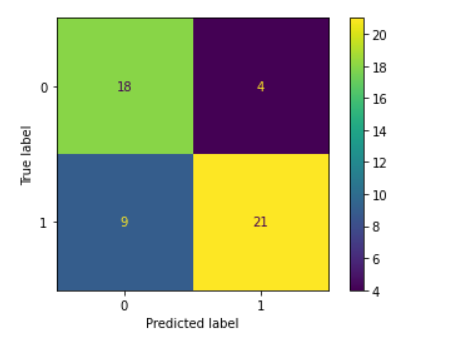
\includegraphics[width=0.45\textwidth, height=130px]{images/naivebayesconfmat.png}}
	\hspace{5pt}
	\subcaptionbox{Naive Bayes ROC curve}{
		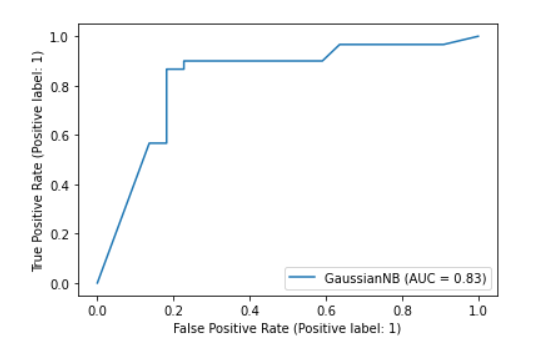
\includegraphics[width=0.45\textwidth, height=130px]{images/naivebayesauc.png}}
	\caption{Naive Bayes overall performance}
	\label{fig:naive_bayes_perf}
\end{figure}
For the Naive Bayes algorithm we can see that the mean absolute error is quite high, the
difference between the training set accuracy and testing set accuracy is more than 10 percent, the f1-score
is quite low and the ROC curve isn't the best.
\\[5pt]
\begin{figure}[H]
	\centering
	\subcaptionbox{SVC performance scores}{
		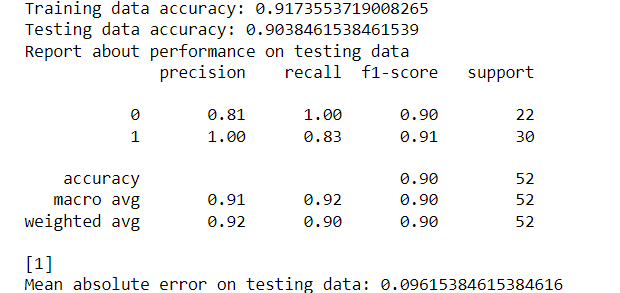
\includegraphics[width=0.45\textwidth, height=130px]{images/svmperf.png}}
	\hspace{5pt}
	\subcaptionbox{SVC confusion matrix}{
		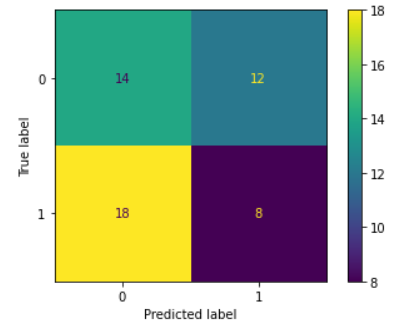
\includegraphics[width=0.45\textwidth, height=130px]{images/svmconfmat.png}}
	\hspace{5pt}
	\subcaptionbox{SVC ROC curve}{
		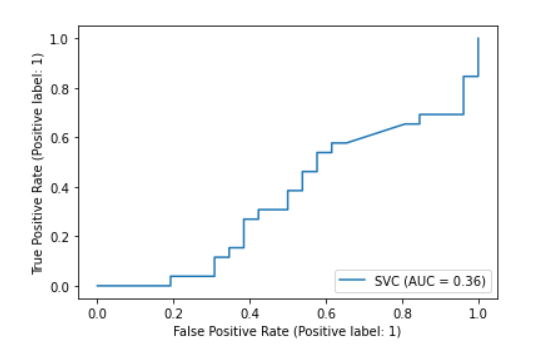
\includegraphics[width=0.45\textwidth, height=130px]{images/svmauc.png}}
	\caption{SVC overall performance}
	\label{fig:svc_perf}
\end{figure}
Now for the SVC algorithm we can see perfect scores in case of precision, which is impossible to be 1.0
, meaning that we might have an overfitting problem. But, other than precision the other scores show us a promising
model until we watch the confusion matrix and the ROC curve. We can see that the confusion matrix is giving us more false predicted
values than it should have, meaning that most of the predictions the model made were false predictions. Not only confusion matrix is
giving us a red light for this model, but even the AUC value which is showing us an awful result, where most of the points are below the
middle point.
\\[5pt]
\begin{figure}[H]
	\centering
	\subcaptionbox{Logistic regression performance scores}{
		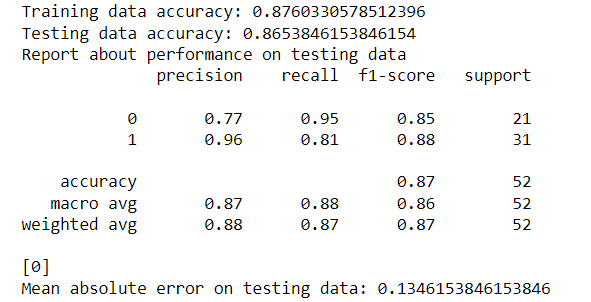
\includegraphics[width=0.45\textwidth, height=130px]{images/scores_model.png}}
	\hspace{5pt}
	\subcaptionbox{Logistic regression confusion matrix}{
		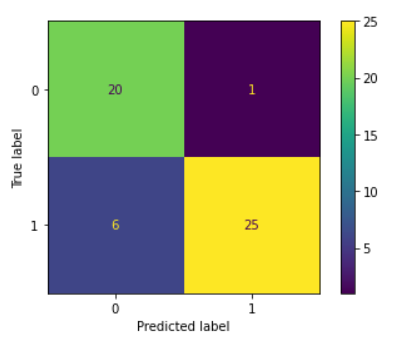
\includegraphics[width=0.45\textwidth, height=130px]{images/confusion_matrix.png}}
	\hspace{5pt}
	\subcaptionbox{Logistic regression ROC curve}{
		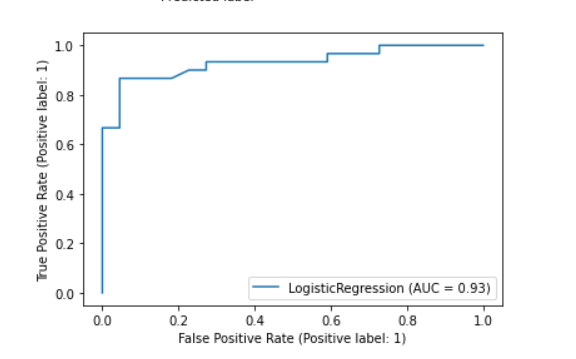
\includegraphics[width=0.45\textwidth, height=130px]{images/Roc_curve_model.png}}
	\caption{Logistic regression overall performance}
	\label{fig:lgs_perf}
\end{figure}
However, if we take a look at the Logistic regression algorithm performance then we can see
a good accuracy on both, training set and testing set, with a difference of 1.1 percent.
Besides the accuracy we see a good recall and precision score, which makes a good f1 score.
The confusion matrix tells us that the most of the values predicted are true, and the ROC curve
shows us a very good AUC score of 0.93.
\subsection{Passing account's data to model}
As it was mentioned in \ref{ss:acc_data}, the function responsible for fetching data returns a dictionary of
multiple data fields for the account. In order to pass the data we first need to filter them and get the fields
that are relatable to our model. 
\\[5pt]
\begin{lstlisting}[language=python, caption={Method that returns the model decision}, captionpos=b]
	def modelDecision(self, account_data):
		dataForModel = {}
		dataForModel['followers'] = int(account_data['followers_count'])
		dataForModel['followings'] = int(account_data['following_count'])
		dataForModel['statuses'] = account_data['statuses_count']
		dataForModel['profile'] = 1 if 'missing' not in account_data['avatar'].split('/') else 0
		dataForModel['server'] = account_data['url'].split('/')[2]
		dataForModel['dateOfCreation'] = int(str(account_data['created_at']).split('-')[0])
		data = []
		for index, feature in enumerate(self.features):
			if index < 4:
				data.append(dataForModel[feature])
			elif index > 3 and index < 11:
				if feature == dataForModel['server']:
					data.append(1)
				else:
					data.append(0)
			else:
				if feature == dataForModel['dateOfCreation']:
					data.append(1)
				else:
					data.append(0)
	
		model_result = bool(self.model.predict([data])[0])
		print(model_result)
		return model_result
\end{lstlisting}
The method \textbf{modelDecision} filters the data to the ones that are relatable to our model and
afterwards uses those data to predict the result, which is type converted from integer to boolean, and then
returned as a boolean in the end.
\section{Database}
We used database in our application in order to save the already checked users and domains. For the database
we chose to use the \textbf{SQLite} \cite{sqlite} with it's API Python library called \textbf{sqlite3} \cite{sqllite3}.
\\[5pt]
We created two tables, one for the handled accounts and one for the handled domains. They are both initialized at the same time
and they are not connected with each other, meaning that they behave independently.
\\[5pt]
As a first step of initializing the database is to connect to it, create the tables and after we are done we need to commit the data.
\subsection{Handled accounts table}\label{ss:hand_acc}
The handled accounts table consists of these data:
\begin{itemize}
	\item \textbf{Account id}, as a primary key.
	\item \textbf{Account username}
	\item \textbf{Account domain}
	\item \textbf{Threat boolean}
\end{itemize}
So, whenever an account is getting checked for the threat possibility, it will immediately go in the database
after the threat possibility result is given, and that account doesn't need to be checked twice since it's in the database
of the handled accounts already.
\subsection{Handled domains table}
The handled domain table consists of these data:
\begin{itemize}
	\item \textbf{Domain name}, as a primary key.
	\item \textbf{Blocked boolean}
\end{itemize}
In case of the domain, we insert it the moment we know the action the user has taken against it, since we need to know whether the user blocked it or not.
\section{Graphical user interface}
This application uses a very simple GUI, with the aim that the user cannot do any big mistake during runtime.
Since, it is planned to run on the background we valued the program safety during the runtime more than the design
itself.
\\[5pt]
The library we used for the GUI is \textbf{Tkinter} \cite{tkinter}, which is provided by Python for desktop applications containing many
useful elements. In order to read the images we used \textbf{Pillow} \cite{pil}.
\\[5pt]
Our GUI consists of a front-end and a back-end part, where the front-end is responsible for displaying the state of the action
executions and the program. Whereas, the back-end is responsible for the whole logic behind predicting whether an account has
the possibility of the threat or not.
\\[5pt]
It is worth mentioning that the whole GUI is not resizable, meaning that there is one permanent size, and this is done for the reason
that the user needs the GUI to be as small as possible but well visible, because he will run it on the background.
\\[5pt]
During the front-end our main problem was updating the window constantly since our application has some loops and the Tkinter
built-in function \textbf{mainloop} is a loop itself. Even when we wanted to initialize the API and the database, there were a few
seconds taken while being executed, meaning that we had to start a separate thread to initialize it while the window is being updated constantly until the initialization is completed.
\\[5pt]
The thread was created by using the \textbf{Threading} \cite{thread} Python module.
\\[5pt]
\begin{lstlisting}[language=python, caption={Updating window while initializing the API and database}, captionpos=b]
	def initAppReq(self):
		try:
			self.app = Application(self.username, self.password, self.server)
			self.app.initApi()
			self.done_init = True
		except Exception:
			self.widgets['main'][7]['state'] = tk.NORMAL
			if('elte.hu' not in self.server and '@' not in self.username):
				showerror(message="You should enter your email "
									+ "instead of your username "
									+ "since the server is not "
									+ "mastodon.elte.hu")
			else:
				showerror(message="Invalid credentials for mastodon account")
	
	def startApp(self):
		self.widgets['main'][7]['state'] = tk.DISABLED
		self.update()
		init_thread = Thread(target=self.initAppReq, daemon=True)
		init_thread.start()
		while not self.done_init:
			self.update()
			if self.done_init:
				break
			self.update()
		self.app.initDatabase()
		init_thread.join()
		self.update()
		showinfo(message="You are now logged in")
		self.runningScreen()
		self.protocol('WM_DELETE_WINDOW', self.stopApp)
		self.callSession()
\end{lstlisting}
As well as some of our API calls required a waiting time as mentioned in \ref{ss:rate_lim},
so we scheduled them and made an inner loop that updated the window constantly until the API call was executed.
\\[5pt]
\begin{lstlisting}[language=python, caption={Updating the window while calling API functions}, captionpos=b]
	def callSession(self):
		while True:
			self.update()
			print("running")
			try:
				self.accounts_reaching_user = []
				self.after(2400, self.sendRequest)
				self.waitTime(2.6)
				
				if len(self.accounts_reaching_user) > 0:
					for account in self.accounts_reaching_user:
						self.update()
						threat_checked_account = self.app.isItThreat(account)
						account_data = threat_checked_account[0]
						account_name = account_data['username']
						threat_data = threat_checked_account[1]
						domain = account_data['url'].split('/')[2]
						if threat_data:
							message = ("Account: " + account_name
										+ "\nFrom domain: " + domain 
										+ "\nMay be a threat!\nTake action!")
							showinfo(message=message)
				
						self.done = False
				
						self.cleanRunning() 
						self.createAction(account_data, threat_data)
	 		
						while not self.done:
							self.update()
							if self.done:
								break
						self.cleanAction()
				self.app.insertAccountInDatabase(account_data, 
												threat_data)
			except Exception:
				print("Error")
\end{lstlisting}
Our application has three screens in total, which are:
\begin{itemize}
	\item Starting Screen
	\item Running Screen
	\item Action Screen
\end{itemize}
The approach we took to switch between screens is to draw them when it is needed and
clear them if it isn't needed.
\\[5pt]
All the screen elements are saved in a dictionary created at the GUI initialization where the keys
describe the screens and the values are list containing the widgets of each screen.
\\[5pt]
Below we can see the functions that handles this approach.
\\[5pt]
\begin{lstlisting}[language=python, caption={Switching from starting screen to running screen}, captionpos=b]
	def runningScreen(self):
		for widget in self.widgets['main']:
			widget.pack_forget()
		for widget in self.widgets['running']:
			widget.pack()
\end{lstlisting}
Switching between the starting screen to the running screen is done by removing the widgets of the starting screen and initializing
the ones in the running screen.
\\[5pt]
\begin{lstlisting}[language=python, caption={Switching from running screen to action screen}, captionpos=b]
	 def cleanRunning(self):
		for widget in self.widgets['running']:
			widget.pack_forget()
	
	def createAction(self, account_data, threat_data):
		self.canvas.pack_forget()
		self.action_label1 = tk.Label(self, text="Account Action", 
									font=('Ariel', 14), bg='light blue')
		self.widgets['action'].add(self.action_label1)
		self.action_label1.pack()
		
		self.string_var = tk.StringVar()
		self.action_combobox = Combobox(self, 
		textvariable=self.string_var)
		
		self.action_combobox['values'] = ("Trust", 
										"Block",
										"Mute")
		self.action_combobox.current(0)
		self.widgets['action'].add(self.action_combobox)
		self.action_combobox.pack()
		
		self.action_label2 = tk.Label(self, text="Domain Action", 
									font=('Ariel', 14), bg='light blue')
		
		self.widgets['action'].add(self.action_label2)
		self.action_label2.pack()
		
		self.string_var2 = tk.StringVar()
		self.domain_combobox = Combobox(self, 
									textvariable=self.string_var2)
		self.domain_combobox['values'] = ("Trust", 
										"Block")
		self.domain_combobox.current(0)
		self.widgets['action'].add(self.domain_combobox)
		self.domain_combobox.pack()
		
		self.empty_label3 = tk.Label(self, bg='light blue')
		self.widgets['action'].add(self.empty_label3)
		self.empty_label3.pack()
		
		self.action_button = tk.Button(self, 
								text='Take action', 
								command=lambda:
								self.takeAction(account_data, threat_data))
		
		self.widgets['action'].add(self.action_button)
		self.action_button.pack()
		self.canvas.pack()
\end{lstlisting}
Switching from running screen to action screen is done by removing the running screen widgets and creating the elements 
of the action screen and packing them in the frame.
\\[5pt]
\begin{lstlisting}[language=python, caption={Switching from action screen to running screen}, captionpos=b]
	def cleanAction(self):
		for widget in self.widgets['action']:
			widget.destroy()
		self.widgets['action'].clear()
		for widget in self.widgets['running']:
			widget.pack()
\end{lstlisting}
And the other way around, switching from action screen to running screen is done by simply destroying the widgets as objects and clearing the list
under which they were saved, and afterwards packing the running widgets to the frame.
\section{Testing}
To test our application we used \textbf{unit testing} and \textbf{manual testing}.
Running the unit tests was done by the \textbf{Pytest} \cite{pytest} framework, but the run was done in
the CI build and not locally, so the test success can be checked in the git repository (see \ref{s:installation_guide}), under
details in CI build.
\\[5pt]
For the CI we chose to go with \textbf{CircleCI} \cite{ci}
\\[5pt]
\begin{figure}[H]
	\centering
	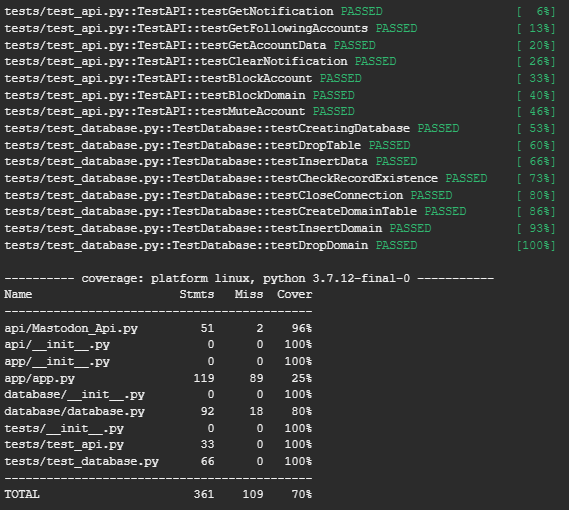
\includegraphics[width=0.8\textwidth,height=250px]{images/test_score2.png}
	\caption{Test coverage and success}
	\label{fig:test_data}
\end{figure}
Our unit test coverage was 70 percent, and the other 30 are functions that depend on user behavior, so they were tested manually.
We applied unit tests on both, API and database, in order to have a quality product.
\\[5pt]
We had the test stored separately for database and API, but they were both tested outside their own class, because
in order to run the tests using Pytest the Python file must have the name test in the beginning or in the end, and the
same applies to the testing method.
\\[5pt]
\begin{lstlisting}[language=python, caption={Example method to test a unit}, captionpos=b]
 	def testCloseConnection(self):
		database = Database()
		database.dropAccountTable()
		database.createTableAccounts()

		id = 1234123
		user = 'Dion'
		domain = 'gibberish'
		threat = False

		database.insertAccount(id, user, domain, threat)

		assert True == database.closeConnection()

		for _ in range(3):
		assert False == database.closeConnection()
\end{lstlisting}
Hence, we did two separate files, one carries the testing of the database and the other one carries the API testing, but
both of the files are under the same directory called testing.
\\[5pt]
We also tested the code style using the \textbf{Flake8} \cite{flake} library, which checks your code base against the \textbf{PEP8} \cite{pep} coding
style.
\subsection{Manual testing}
Some of the units were dependent on user behavior so we manually tested them. In addition, we tested the 
GUI functionality manually as well, to ensure that we are delivering a fast and a non-crashing GUI.
Besides those, the switching between screens was tested, the account information window (see \ref{fig:possible_threat_notification}), action taking fields (see \ref{fig:action_page}) in the action
screen.


